%% LaTeX Beamer presentation template (requires beamer package)
%% see http://bitbucket.org/rivanvx/beamer/wiki/Home
%% idea contributed by H. Turgut Uyar
%% template based on a template by Till Tantau
%% this template is still evolving - it might differ in future releases!

\documentclass[10pt]{beamer}

\mode<presentation>
{
\usetheme{Malmoe}

\setbeamercovered{transparent}
}


\addtobeamertemplate{navigation symbols}{}{%
\usebeamerfont{footline}%
\usebeamercolor[fg]{footline}%
\hspace{1em}%
\insertframenumber/\inserttotalframenumber
}

\usepackage[brazil]{babel}
\usepackage[utf8]{inputenc}

% font definitions, try \usepackage{ae} instead of the following
% three lines if you don't like this look
\usepackage{mathptmx}
\usepackage[scaled=.90]{helvet}
\usepackage{courier}


\usepackage[T1]{fontenc}

\title{Cálculo do número de instruções dos \textit{benchmarks} e implementação
de novas \textit{pin tools}}

%\subtitle{}

% - Use the \inst{?} command only if the authors have different
%   affiliation.
%\author{F.~Author\inst{1} \and S.~Another\inst{2}}
\author{Gustavo Ciotto Pinton}

% - Use the \inst command only if there are several affiliations.
% - Keep it simple, no one is interested in your street address.
\institute
{

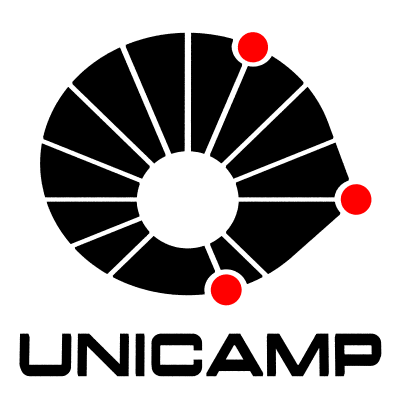
\includegraphics[scale=0.12]{logo} \\
\vspace{16pt}
Universidade Estadual de Campinas - UNICAMP\\
MO601B - Arquitetura de Computadores}

\date{19 de Setembro de 2016}



% If you have a file called "university-logo-filename.xxx", where xxx
% is a graphic format that can be processed by latex or pdflatex,
% resp., then you can add a logo as follows:

% \pgfdeclareimage[height=0.5cm]{university-logo}{university-logo-filename}
% \logo{\pgfuseimage{university-logo}}



% Delete this, if you do not want the table of contents to pop up at
% the beginning of each subsection:
\AtBeginSubsection[]
{
\begin{frame}<beamer>
\frametitle{Outline}
\tableofcontents[currentsection,currentsubsection]
\end{frame}
}

% If you wish to uncover everything in a step-wise fashion, uncomment
% the following command:

%\beamerdefaultoverlayspecification{<+->}

\begin{document}

\begin{frame}

\titlepage
\end{frame}

\section{Contagem de instruções dos benchmarks}


\begin{frame}
\frametitle{Contagem de instruções dos \textit{benchmarks}}
\framesubtitle{Escolha da \textit{pin tool}}

\begin{itemize}
  \item \textit{Tools} disponíveis para a contagem de instruções:
  \begin{itemize}
    \item \texttt{inscount0}: Nenhuma otimização. Funções de rotina inseridas a
    cada instrução.
    \item \texttt{inscount1}: medida de granularidade é o BBL (\textit{basic
    block}), economizando diversas chamadas à função de análise.
    \item \texttt{inscount2}: BBL, inserção \texttt{IPOINT\_ANYWHERE} e
    \texttt{PIN\_FAST\_ANALYSIS\_CALL};
    \item \texttt{inscount\_tls}: BBL, inserção \texttt{IPOINT\_ANYWHERE},
    \texttt{PIN\_FAST\_ANALYSIS\_CALL} e unidade de armazenamento rápido,
    \texttt{TLS}, indexado pelos \textit{ids} das threads.
  \end{itemize}
  \vspace{12pt}
  \item Melhor performance para o nosso caso: \texttt{inscount2}!
  \begin{itemize}
    \item Não são necessárias informações sobre o número de \textit{threads};
    \item Aproximadamente 20 horas para um Intel i3.
  \end{itemize}
\end{itemize}
\end{frame}

\begin{frame}
\frametitle{Contagem de instruções dos \textit{benchmarks}}
\framesubtitle{Resultados}

\begin{figure}[h!]
\centering
\centering
\label{fig:cint}
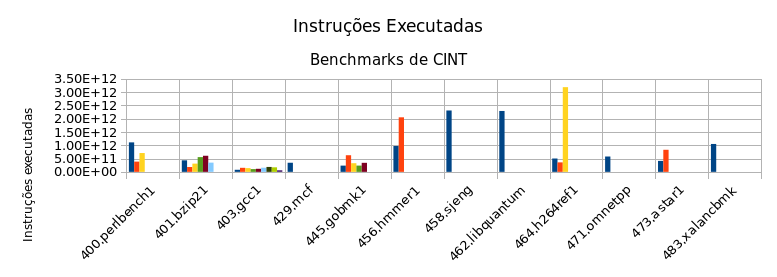
\includegraphics[width=0.9\linewidth]{cint}
\caption{Número de instruções dos \textit{benchmarks} pertencentes ao conjunto \texttt{CINT}.}
\end{figure}

\end{frame}

\begin{frame}
\frametitle{Contagem de instruções dos \textit{benchmarks}}
\framesubtitle{Resultados}

\begin{figure}[h!]
\centering
\label{fig:cfp}
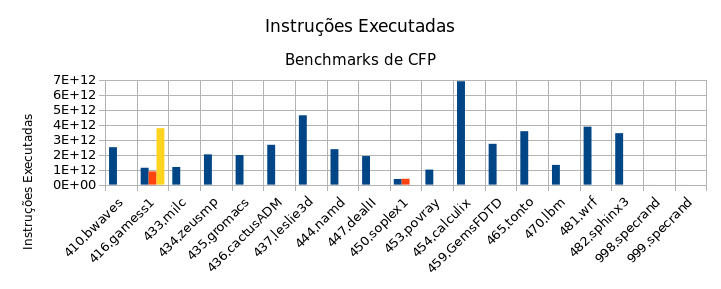
\includegraphics[width=0.9\linewidth]{cfp}
\caption{Número de instruções dos \textit{benchmarks} pertencentes ao conjunto \texttt{CFP}.}
\end{figure}
\end{frame}

\begin{frame}
\frametitle{Contagem de instruções dos \textit{benchmarks}}
\framesubtitle{Resultados}

\begin{itemize}
  \item \texttt{403.gcc} utiliza mais entradas em
  seus testes, com 9 entradas, totalizando 1.152.387.847.873
  instruções executadas;
  \vspace{12pt}
  \item \texttt{454.calculix} : maior número de  instruções com
  6.894.341.859.256;
  \vspace{12pt}
  \item \texttt{998.specrand} e \texttt{999.specrand}: mesmo número de
  instruções (536.611.748 instruções cada);
  \vspace{12pt}
  \item Em geral, os \textit{benchmarks} do conjunto inteiro executam menos instruções
  que os do conjunto de ponto flutuante.
\end{itemize}

\end{frame}

\begin{frame}
\frametitle{Implementação de novas \textit{pin tools}}

\begin{itemize}
  \item Contagem do número de instruções por rotina e por \textit{thread};
  \begin{itemize}
    \item Função de instrumentação: a cada \textbf{rotina};
    \item Função de análise: a cada \textbf{instrução}.
    \item 2 listas ligadas: 1 de rotinas e outra de \textit{threads}:
    \item Cada nó de rotina contém \textit{nome} (\texttt{RTN\_Name}),
    \textit{id} (\texttt{RTN\_Id}), o primeiro nó de uma lista de
    \textit{threads} e um ponteiro para o próximo nó;
    \item Cada nó de \textit{thread} contém a sua \textit{id}
    (\texttt{THREAD\_ID}), o número de instruções executadas da respectiva
    rotina e um ponteiro para o próximo nó;
    \item Programas com muitas \textit{threads}: forte impacto negativo à
    performance, uma vez que um nó de \textit{thread} é procurado a cada
    instrução (rotina de análise).
  \end{itemize}
  
\end{itemize}

\end{frame}

\begin{frame}
\frametitle{Implementação de novas \textit{pin tools}}

\begin{itemize}
  \item Simulação de dois modelos de \textit{branch prediction} discutidos em
  aula (1 e 2 \textit{bits}).
  
  \begin{itemize}
    \item Função de instrumentação: a cada \textbf{instrução};
    \item Função de análise: a cada \textbf{instrução} de \textit{branch} ou
    chamada de rotina.
    
    \vspace{12pt}
    \item Função \textit{hash}: 12 \textit{bits} menos significativos;
    \vspace{12pt}
    \item Modelo de \textit{1 bit}: apenas o último salto é considerado;
    \item Modelo de \textit{2 bits}: máquina de estados com 4 estados
    (\texttt{STRONG\_TAKEN}, \texttt{WEAK\_TAKEN}, \texttt{STRONG\_NOT\_TAKEN}
    e \texttt{WEAK\_NOT\_TAKEN}).
    
  \end{itemize}
  \vspace{12pt}
  \item Testes no conjunto \texttt{ref} dos \textit{benchmarks} \texttt{400.perlbench}, \texttt{401.bzip2},
  \texttt{403.gcc}, \texttt{445.gobmk} e \texttt{999.specrand}
  
\end{itemize}

\end{frame}

\begin{frame}
\frametitle{Implementação de novas \textit{pin tools}}
\framesubtitle{Resultados}

\begin{itemize}
  \item Contagem do número de instruções por rotina e por \textit{thread}:
  \begin {itemize}
    \item\textit{Benchmarks} \textbf{testados} apresentam apenas uma
    \textit{thread}: performance não é \textit{extremamente}
    degradada;
    
  \end{itemize}
  \end{itemize}
  \begin{table}[h]
\centering
\caption{\label{tab:modelos} Resultados obtidos para algumas rotinas
importantes.}
\begin{tabular}{| c | c | c | c |}
\hline

\textit{\textbf{Benchmark}} & \textit{E}  & \textit{Rotina} & \% \\	\hline \hline
\texttt{400.perlbench} & 3 & \texttt{S\_regmatch} & 50 \\\hline
\texttt{401.bzip2} & 6 & \texttt{BZ2\_compressBlock} & 22.2 \\ \hline
\texttt{403.gcc} & 9 & \texttt{bitmap\_operation} & 9.2 \\ \hline
\texttt{445.gobmk} & 5 & \texttt{do\_play\_move} & 8.4 \\ \hline
\texttt{999.specrand} & 1 &  \texttt{GI\_\_printf\_fp} & 32.6\\ \hline
\end{tabular}
\end{table}


\end{frame}

\begin{frame}
\frametitle{Implementação de novas \textit{pin tools}}
\framesubtitle{Resultados}

\begin{itemize}

    \item Simulação de dois modelos de \textit{branch prediction} discutidos em
    aula (1 e 2 \textit{bits}).
  \end{itemize}
  
{\scriptsize 
  \begin{table}[h]
\centering
\caption{\label{tab:modelos} Resultados obtidos para os modelos \textit{1-bit}
e \textit{2-bit}.}
\begin{tabular}{| c | c | c | c | c | c | c | c |}

\hline
\multicolumn{2}{|c|}{} & \multicolumn{3}{c|}{\textbf{Modelo 1}} &
\multicolumn{3}{|c|}{\textbf{Modelo 2}}	\\ 	\hline
\textit{\textbf{Benchmark}} & \textit{E}  & \textit{Misses} & \textit{Hits} &
\% & \textit{Misses} & \textit{Hits} & \% \\
\hline \hline \texttt{400.perlbench} & 3 & \(4.0\times10^{10}\) &
\(9.4\times10^{10}\) & 0.70 & \(2.7\times10^{10}\) & \(1.1\times10^{11}\)
& 0.80 \\
\hline \texttt{401.bzip2} & 6 & \(9.1\times10^{9}\) & \(5.4\times10^{10}\) &
0.86 & \(1.3\times10^{10}\) & \(5.0\times10^{10}\) & 0. 79 \\ \hline
\texttt{403.gcc} & 9 & \(4.7\times10^{9}\) & \(2.3\times10^{10}\) &
0.83 & \(4.9\times10^{9}\) & \(2.3\times10^{10}\) & 0. 82 \\ \hline
\texttt{445.gobmk} & 5 & \(2.0\times10^{10}\) & \(4.3\times10^{10}\)  & 0.68 &
\(1.8\times10^{10}\) & \(4.5\times10^{10}\) & 0.72 \\ \hline
\texttt{999.specrand} & 1 & \(3.9\times10^{7}\) & \(6.4\times10^{7}\) & 0.62 &
\(4.7\times10^{7}\) & \(5.9\times10^{7}\) & 0.58\\ \hline
\end{tabular}
\end{table}

}
\end{frame}

\end{document}
